\documentclass[tikz,border=8pt,multi=tikzpicture]{standalone}
\usepackage{amsmath}
\usepackage{xcolor}
\usetikzlibrary{arrows.meta, calc}

\definecolor{mainblue}{HTML}{001158}
\definecolor{accent}{HTML}{8592bc}
\definecolor{lightaccent}{HTML}{e7e9f2}

\tikzset{
  force/.style={-{Stealth[length=3mm]}, line width=1.2pt, color=mainblue},
  dim/.style={-{Stealth[length=2mm]}, line width=0.7pt, color=accent},
  moment/.style={-{Stealth[length=2.5mm]}, line width=1.2pt, color=mainblue},
  qload/.style={-{Stealth[length=2mm]}, line width=0.9pt, color=mainblue!70},
  guide/.style={accent, dashed, line width=0.6pt},
  every node/.append style={font=\sffamily}
}

\newcommand{\festlager}[1]{
  \begin{scope}[shift={#1}]
    \draw[line width=1pt] (0,0) -- (-0.3,-0.5) -- (0.3,-0.5) -- cycle;
    \draw[line width=1pt] (-0.42,-0.5) -- (0.42,-0.5);
    \foreach \x in {-0.42,-0.24,...,0.42} {\draw[line width=0.4pt] (\x,-0.5) -- (\x-0.13,-0.68);}
  \end{scope}
}
\newcommand{\loslager}[1]{
  \begin{scope}[shift={#1}]
    \draw[line width=1pt] (0,0) -- (-0.3,-0.5) -- (0.3,-0.5) -- cycle;
    \foreach \x in {-0.18,0,0.18} {\draw[fill=white, line width=0.7pt] (\x,-0.6) circle (0.1);}
    \draw[line width=1pt] (-0.42,-0.72) -- (0.42,-0.72);
    \foreach \x in {-0.42,-0.24,...,0.42} {\draw[line width=0.4pt] (\x,-0.72) -- (\x-0.13,-0.9);}
  \end{scope}
}
\newcommand{\einspannung}[1]{
  \begin{scope}[shift={#1}]
    \draw[mainblue, line width=1.5pt] (0,0.6) -- (0,-0.6);
    \foreach \y in {-0.5,-0.25,...,0.5} {\draw[line width=0.5pt] (0,\y) -- (-0.25,\y+0.22);}
  \end{scope}
}
\newcommand{\qarrows}[4]{
  \draw[mainblue!70, line width=0.8pt] (#1,#3) -- (#2,#3);
  \pgfmathsetmacro{\qn}{int(round((#2-#1)/0.5))}
  \foreach \i in {0,...,\qn} {
    \pgfmathsetmacro{\qx}{(#1)+\i*0.5}
    \draw[qload] (\qx,#3) -- (\qx,#3-#4);
  }
}

\begin{document}

% ================= Concept: sign convention for N, V, M =================
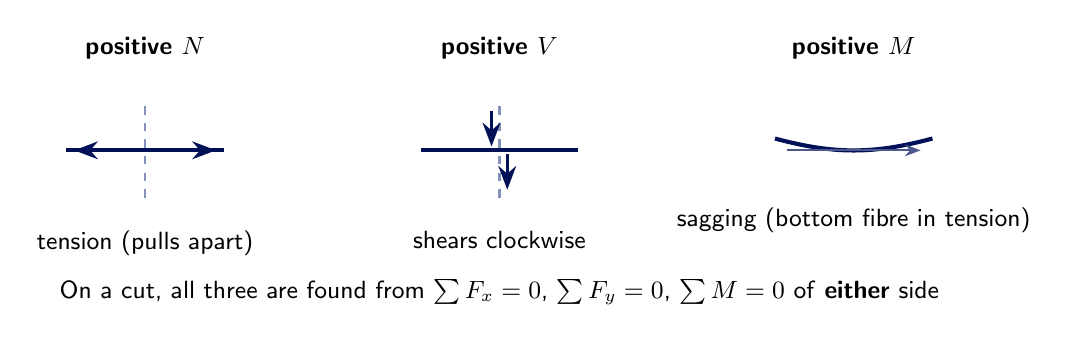
\begin{tikzpicture}
% --- N ---
\node[align=center] at (0,1.3) {\small \textbf{positive $N$}};
\draw[mainblue, line width=1.5pt] (-1,0) -- (1,0);
\draw[accent, dashed, line width=0.8pt] (0,-0.6) -- (0,0.6);
\draw[force] (0.1,0) -- (0.9,0);
\draw[force] (-0.1,0) -- (-0.9,0);
\node[below] at (0,-0.9) {\small tension (pulls apart)};
% --- V ---
\begin{scope}[shift={(4.5,0)}]
\node[align=center] at (0,1.3) {\small \textbf{positive $V$}};
\draw[mainblue, line width=1.5pt] (-1,0) -- (1,0);
\draw[accent, dashed, line width=0.8pt] (0,-0.6) -- (0,0.6);
\draw[force] (-0.1,0.5) -- (-0.1,0.05);
\draw[force] (0.1,-0.05) -- (0.1,-0.5);
\node[below] at (0,-0.9) {\small shears clockwise};
\end{scope}
% --- M ---
\begin{scope}[shift={(9,0)}]
\node[align=center] at (0,1.3) {\small \textbf{positive $M$}};
\draw[mainblue, line width=1.5pt] (-1,0.15) to[out=-15,in=195] (1,0.15);
\draw[qload, line width=0.8pt] (-0.85,0.0) -- (0.85,0.0);
\node[below] at (0,-0.6) {\small sagging (bottom fibre in tension)};
\end{scope}
\node[align=center] at (4.5,-1.8) {\small On a cut, all three are found from $\sum F_x=0$, $\sum F_y=0$, $\sum M=0$ of \textbf{either} side};
\end{tikzpicture}

% ================= Ex 9.1 problem: simply supported beam, point load =================
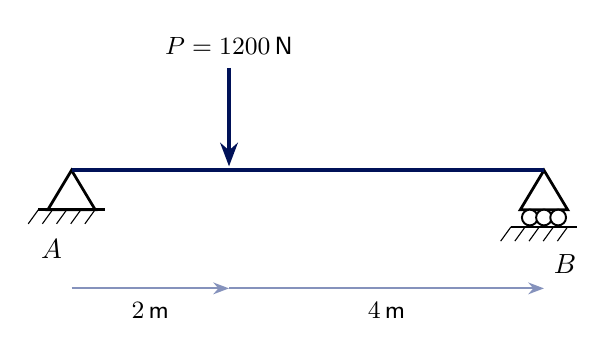
\begin{tikzpicture}
\festlager{(0,0)}
\loslager{(6,0)}
\draw[mainblue, line width=1.5pt] (0,0) -- (6,0);
\node[below left] at (0,-0.75) {$A$};
\node[below right] at (6,-0.95) {$B$};
\draw[force] (2,1.3) -- (2,0.05);
\node[above] at (2,1.35) {\small $P=1200\,\text{N}$};
\draw[dim] (0,-1.5) -- (2,-1.5);
\node[below] at (1,-1.55) {\small $2\,\text{m}$};
\draw[dim] (2,-1.5) -- (6,-1.5);
\node[below] at (4,-1.55) {\small $4\,\text{m}$};
\end{tikzpicture}

% ================= Ex 9.1 solution: beam + V(x) + M(x) =================
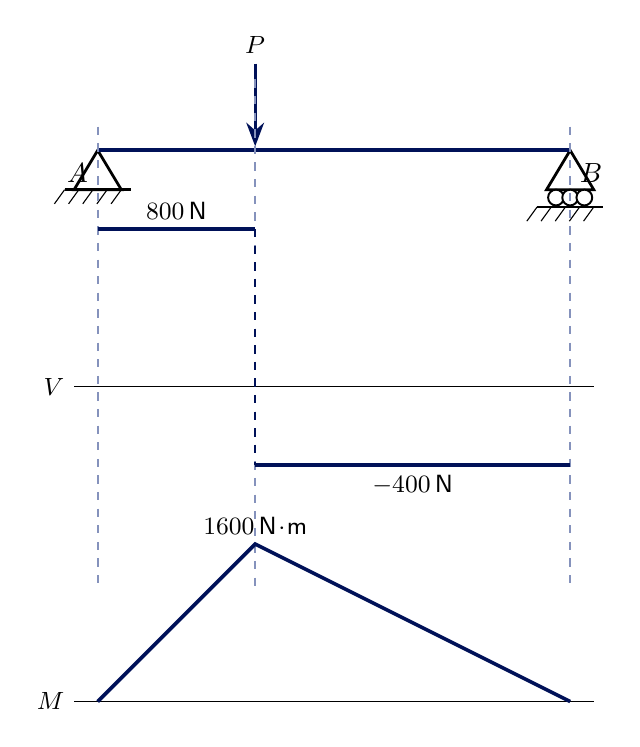
\begin{tikzpicture}
\festlager{(0,0)}
\loslager{(6,0)}
\draw[mainblue, line width=1.5pt] (0,0) -- (6,0);
\draw[force] (2,1.1) -- (2,0.05);
\node[above] at (2,1.1) {\small $P$};
\node[below left] at (0,-0.05) {$A$};
\node[below right] at (6,-0.05) {$B$};
\draw[guide] (0,0.3) -- (0,-5.6);
\draw[guide] (2,0.9) -- (2,-5.6);
\draw[guide] (6,0.3) -- (6,-5.6);
% V diagram, baseline y=-3
\node[left] at (-0.3,-3) {\small $V$};
\draw[line width=0.6pt] (-0.3,-3) -- (6.3,-3);
\draw[mainblue, line width=1.3pt] (0,-1) -- (2,-1);
\draw[mainblue, dashed, line width=0.8pt] (2,-1) -- (2,-4);
\draw[mainblue, line width=1.3pt] (2,-4) -- (6,-4);
\node[above] at (1,-1) {\small $800\,\text{N}$};
\node[below] at (4,-4) {\small $-400\,\text{N}$};
% M diagram, baseline y=-7
\node[left] at (-0.3,-7) {\small $M$};
\draw[line width=0.6pt] (-0.3,-7) -- (6.3,-7);
\draw[mainblue, line width=1.3pt] (0,-7) -- (2,-5) -- (6,-7);
\node[above] at (2,-5) {\small $1600\,\text{N}\!\cdot\!\text{m}$};
\end{tikzpicture}

% ================= Ex 9.2 problem: cantilever, tip load =================
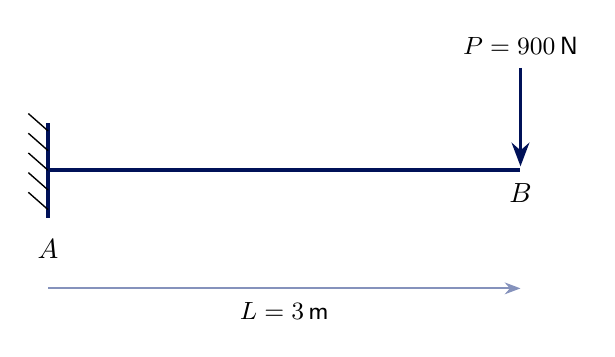
\begin{tikzpicture}
\einspannung{(0,0)}
\draw[mainblue, line width=1.5pt] (0,0) -- (6,0);
\node[below] at (0,-0.75) {$A$};
\node[below] at (6,-0.05) {$B$};
\draw[force] (6,1.3) -- (6,0.05);
\node[above] at (6,1.35) {\small $P=900\,\text{N}$};
\draw[dim] (0,-1.5) -- (6,-1.5);
\node[below] at (3,-1.55) {\small $L=3\,\text{m}$};
\end{tikzpicture}

% ================= Ex 9.2 solution: beam + V(x) + M(x) =================
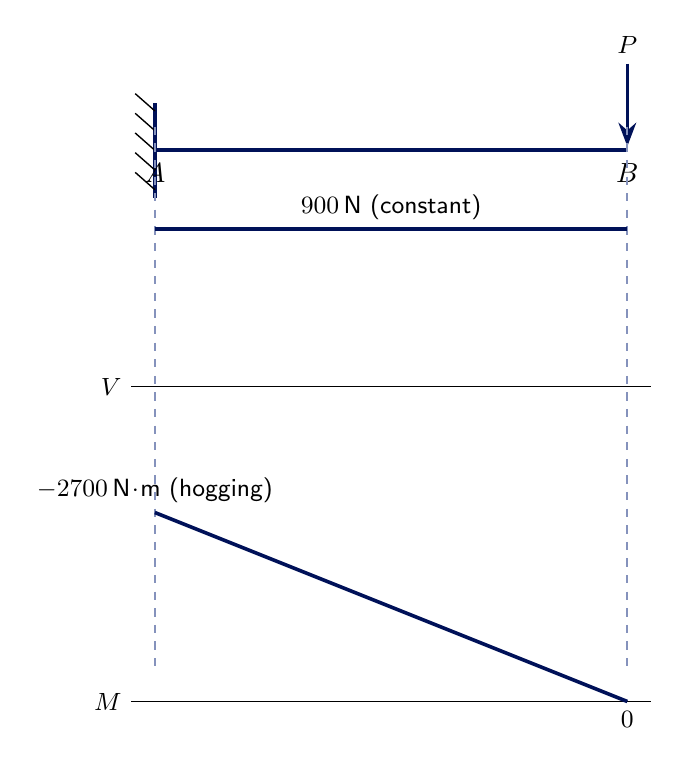
\begin{tikzpicture}
\einspannung{(0,0)}
\draw[mainblue, line width=1.5pt] (0,0) -- (6,0);
\draw[force] (6,1.1) -- (6,0.05);
\node[above] at (6,1.1) {\small $P$};
\node[below] at (0,-0.05) {$A$};
\node[below] at (6,-0.05) {$B$};
\draw[guide] (0,0.3) -- (0,-6.6);
\draw[guide] (6,0.3) -- (6,-6.6);
% V diagram, baseline y=-3
\node[left] at (-0.3,-3) {\small $V$};
\draw[line width=0.6pt] (-0.3,-3) -- (6.3,-3);
\draw[mainblue, line width=1.3pt] (0,-1) -- (6,-1);
\node[above] at (3,-1) {\small $900\,\text{N}$ (constant)};
% M diagram, baseline y=-7, negative (hogging) so drawn above its own baseline
\node[left] at (-0.3,-7) {\small $M$};
\draw[line width=0.6pt] (-0.3,-7) -- (6.3,-7);
\draw[mainblue, line width=1.3pt] (0,-4.6) -- (6,-7);
\node[above] at (0,-4.6) {\small $-2700\,\text{N}\!\cdot\!\text{m}$ (hogging)};
\node[below] at (6,-7) {\small $0$};
\end{tikzpicture}

% ================= Ex 9.3 problem: simply supported beam, full UDL =================
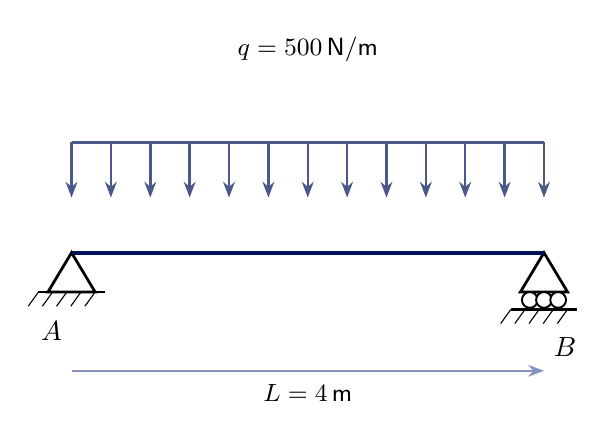
\begin{tikzpicture}
\festlager{(0,0)}
\loslager{(6,0)}
\draw[mainblue, line width=1.5pt] (0,0) -- (6,0);
\node[below left] at (0,-0.75) {$A$};
\node[below right] at (6,-0.95) {$B$};
\qarrows{0}{6}{1.4}{0.7}
\node[above] at (3,2.3) {\small $q=500\,\text{N/m}$};
\draw[dim] (0,-1.5) -- (6,-1.5);
\node[below] at (3,-1.55) {\small $L=4\,\text{m}$};
\end{tikzpicture}

% ================= Ex 9.3 solution: beam + V(x) linear + M(x) parabola =================
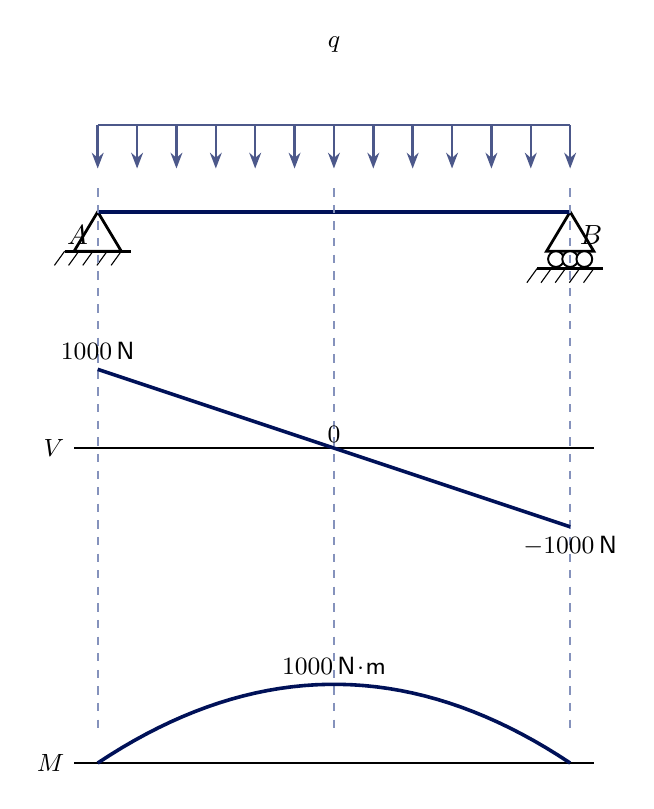
\begin{tikzpicture}
\festlager{(0,0)}
\loslager{(6,0)}
\draw[mainblue, line width=1.5pt] (0,0) -- (6,0);
\qarrows{0}{6}{1.1}{0.55}
\node[above] at (3,1.9) {\small $q$};
\node[below left] at (0,-0.05) {$A$};
\node[below right] at (6,-0.05) {$B$};
\draw[guide] (0,0.3) -- (0,-6.6);
\draw[guide] (3,0.3) -- (3,-6.6);
\draw[guide] (6,0.3) -- (6,-6.6);
% V diagram, baseline y=-3, linear from +1 to -1 (scale: 1 unit = 1000 N)
\node[left] at (-0.3,-3) {\small $V$};
\draw[line width=0.6pt] (-0.3,-3) -- (6.3,-3);
\draw[mainblue, line width=1.3pt] (0,-2) -- (6,-4);
\node[above] at (0,-2) {\small $1000\,\text{N}$};
\node[below] at (6,-4) {\small $-1000\,\text{N}$};
\node[above] at (3,-3.05) {\small $0$};
% M diagram, baseline y=-7, parabola (scale: 1 unit = 1000 N*m)
\node[left] at (-0.3,-7) {\small $M$};
\draw[line width=0.6pt] (-0.3,-7) -- (6.3,-7);
\draw[mainblue, line width=1.3pt] plot[domain=0:6, samples=40] (\x,{-7+(1-(\x-3)*(\x-3)/9)});
\node[above] at (3,-6) {\small $1000\,\text{N}\!\cdot\!\text{m}$};
\end{tikzpicture}

\end{document}
